\documentclass{article}
\usepackage[T1]{fontenc}
\usepackage{fancyhdr}
\usepackage{extramarks}
\usepackage{amsmath}
\usepackage{amsthm}
\usepackage{amsfonts}
\usepackage{dsfont}
\usepackage{tikz}
\usepackage[plain]{algorithm}
\usepackage{algpseudocode}
\usepackage{graphicx}
\usepackage{listings}

\graphicspath{ {./../img} }

\usetikzlibrary{automata,positioning}

%
% Basic Document Settings
%

\topmargin=-0.45in
\evensidemargin=0in
\oddsidemargin=0in
\textwidth=6.5in
\textheight=9.0in
\headsep=0.25in

\linespread{1.1}

\pagestyle{fancy}
\lhead{\hmwkAuthorName}
\chead{\hmwkTitle}
\rhead{\hmwkClass}
\lfoot{\lastxmark}
\cfoot{\thepage}

\renewcommand\headrulewidth{0.4pt}
\renewcommand\footrulewidth{0.4pt}

\setlength\parindent{0pt}
\setlength{\parskip}{5pt}

%
% Homework Details
%   - Title
%   - Due date
%   - Class
%   - Section/Time
%   - Instructor
%   - Author
%

\newcommand{\hmwkTitle}{Quiz\ \#2}
\newcommand{\hmwkDueDate}{October 30, 2023}
\newcommand{\hmwkClass}{ECE 271A}
\newcommand{\hmwkClassInstructor}{Professor Vasconcelos}
\newcommand{\hmwkAuthorName}{\textbf{Ray Tsai}}
\newcommand{\hmwkPID}{A16848188}

%
% Title Page
%

\title{
    \vspace{2in}
    \textmd{\textbf{\hmwkClass:\ \hmwkTitle}}\\
    \normalsize\vspace{0.1in}\small{Due\ on\ \hmwkDueDate\ at 11:59pm}\\
    \vspace{0.1in}\large{\textit{\hmwkClassInstructor}} \\
    \vspace{3in}
}

\author{
  \hmwkAuthorName \\
  \vspace{0.1in}\small\hmwkPID
}
\date{}

%
% Various Helper Commands
%

% Useful for algorithms
\newcommand{\alg}[1]{\textsc{\bfseries \footnotesize #1}}

% For derivatives
\newcommand{\deriv}[1]{\frac{\mathrm{d}}{\mathrm{d}x} (#1)}

% For partial derivatives
\newcommand{\pderiv}[2]{\frac{\partial}{\partial #1} (#2)}

% Integral dx
\newcommand{\dx}{\mathrm{d}x}

% Probability commands: Expectation, Variance, Covariance, Bias
\newcommand{\Var}{\mathrm{Var}}
\newcommand{\Cov}{\mathrm{Cov}}
\newcommand{\Bias}{\mathrm{Bias}}
\newcommand*{\Z}{\mathbb{Z}}
\newcommand*{\Q}{\mathbb{Q}}
\newcommand*{\R}{\mathbb{R}}
\newcommand*{\C}{\mathbb{C}}
\newcommand*{\N}{\mathbb{N}}
\newcommand*{\prob}{\mathds{P}}
\newcommand*{\E}{\mathds{E}}

\begin{document}

\maketitle

\pagebreak

\section*{Part A}

Using the training data in {\fontfamily{qcr}\selectfont TrainingSampleDCT\textunderscore8.mat} compute the histogram estimate of the prior
$P_Y(i), i \in \{cheetah, grass\}$. Using the results of problem $2$ compute the maximum likelihood estimate
for the prior probabilities. Compare the result with the estimates that you obtained last week. If they
are the same, interpret what you did last week. If they are different, explain the differences.
\\

\textbf{\large Solution}

Let $n$ be the total sample size, $C_j$ be the count of samples for class $j$, and $\pi_j = P_Y(j)$.
To derive the ML estamator for $P_{C_1,\dots,C_N}(c_1,\dots,c_N) = \frac{n!}{\prod_{k = 1}^N c_k!}\prod^N_{j = 1}\pi^{c_j}_j$, given the constraint $\sum^N_j \pi_j = 1$,
we first take the logarithm of $P_{C_1,\dots,C_N}(c_1,\dots,c_N)$ and get
\[
  \ln P_{C_1,\dots,C_N}(c_1,\dots,c_N) = \ln \frac{n!}{\prod_{k = 1}^N c_k!} + \sum^N_{j = 1} c_j \ln \pi_j.
\]
Let $\theta = (\pi_1, \dots, \pi_N)^T$, and let $L(\theta, \lambda) = \ln P_{C_1,\dots,C_N}(c_1,\dots,c_N) + \lambda\left(\sum^N_j \pi_j - 1\right)$.
Then,
\begin{gather*}
  \nabla_{\theta}L = \left(\frac{c_1}{\pi_1},\dots, \frac{c_N}{\pi_N}\right)^T + (\lambda, \dots, \lambda)^T = 0 \\
  \frac{\partial}{\partial \lambda}L = \sum_{j = 1}^N \pi_j - 1 = 0.
\end{gather*}
For $1 \leq j \leq N$, we get $\frac{c_j}{\pi_j} + \lambda = 0$, and so $c_j + \pi_j\lambda = 0$. 
Then, $\sum^N_{j = 1} (c_j + \pi_j\lambda) = n + \lambda = 0$, and thus $ \lambda = -n$. 
We also take the Hessian of $L$. Notice that 
\[
    \frac{\partial^2 L}{\partial \pi_i \partial \pi_j} = \begin{cases}
        -\frac{c_j}{\pi_j^2}, & i = j \\
        0, & i \neq j
    \end{cases},
\]
and so $\nabla^2_{\theta} L = \text{diag}\left(-\frac{c_i}{\pi_i^2}, \dots, -\frac{c_N}{\pi_N^2}\right)$.
Since the Hessian of $L$ is obviously negative definite, the critical point we are looking for is indeed a maximum point.
Therefore, we obtain the ML estamator $\theta^* = \left(\frac{c_1}{n},\dots, \frac{c_N}{n}\right)$.

In the case of {\fontfamily{qcr}\selectfont TrainingSampleDCT\textunderscore8.mat}, there are two classes in total, with $250$ samples of class \textit{cheetah} and $1053$ samples of class \textit{grass}.
By our ML estamator, we get
\begin{align*}
  P_Y(cheetah) = \frac{c_{cheetah}}{n} = \frac{250}{1053 + 250} \approx 0.192 && P_Y(grass) = \frac{c_{grass}}{n} = \frac{1053}{1053 + 250} \approx 0.808.
\end{align*}
This result surprisingly coincides with our estimation last week, implying that our intuitive approach of designating the ratio between the sample sizes of each class as the prior probability is in fact somewhat optimal.

\pagebreak

\section*{Part B}

Using the training data in {\fontfamily{qcr}\selectfont TrainingSampleDCT\textunderscore8.mat}, compute the maximum likelihood estimates
for the parameters of the class conditional densities $P_{X|Y}(x|cheetah)$ and $P_{X|Y}(x|grass)$ under the
Gaussian assumption. Denoting by $X = \{X_1,\dots, X_{64}\}$ the vector of DCT coefficients, create $64$ plots
with the marginal densities for the two classes - $P_{X_k|Y} (x_k|cheetah)$ and $P_{X_k|Y} (x_k|grass)$, $k = 1,\dots, 64$
- on each. Use different line styles for each marginal. Select, by visual inspection, what you think are
the best $8$ features for classification purposes and what you think are the worst $8$ features (you can use
the subplot command to compare several plots at a time). Hand in the plots of the marginal densities
for the best-8 and worst-8 features (once again you can use subplot, this should not require more than
two sheets of paper). In each subplot indicate the feature that it refers to.
\\

\textbf{\large Solution}

We know that the ML estamates for a multivariate Gaussian distribution of class $i$ are
\begin{align*}
  \mu_i = \frac{1}{n}\sum_j x^{(i)}_j && \Sigma_i = \frac{1}{n}\sum_j (x^{(i)}_j - \mu_i)(x^{(i)}_j - \mu_i)^T.
\end{align*}
Suppose that $X \sim N(\mu_i, \Sigma_i)$. By applying the projection matrix, we can transform the $64$-dimension Gaussian distribution onto any desired dimension.
Let $A_k = \frac{a_ka_k^T}{a_k^Ta_k}$ be the projection matrix to the $k$-th dimension unit vector $a_k = (0 \dots 1 \dots 0)$.
Then, we know $A_kx \sim N(A_k\mu_i, A_k\Sigma_iA_k^T)$, and $N(A_k\mu_i, A_k\Sigma_iA_k^T)$ is the projection of the $64$-dimension Gaussian distribution onto the $k$-th unit vector.
Notice that $A_k\mu_i$ simply extracts the $k$-th entry of $\mu_i$, namely $\mu_{i_k}$, which becomes our one dimension mean on the $k$-th dimention. 
Similarly, $A_k\Sigma_iA_k^T$ extracts the entry on the $k$-th row $k$-th column, namely $\Sigma_{i_{kk}}$, which becomes our variance on the $k$-th dimension.
Thus, we obtain the marginal density $P_{X_k|Y}(x_k|i) \sim N(\mu_{i_k}, \Sigma_{i_{kk}})$.

The following are the plots for each of the $64$ features for each class:
\begin{center}
  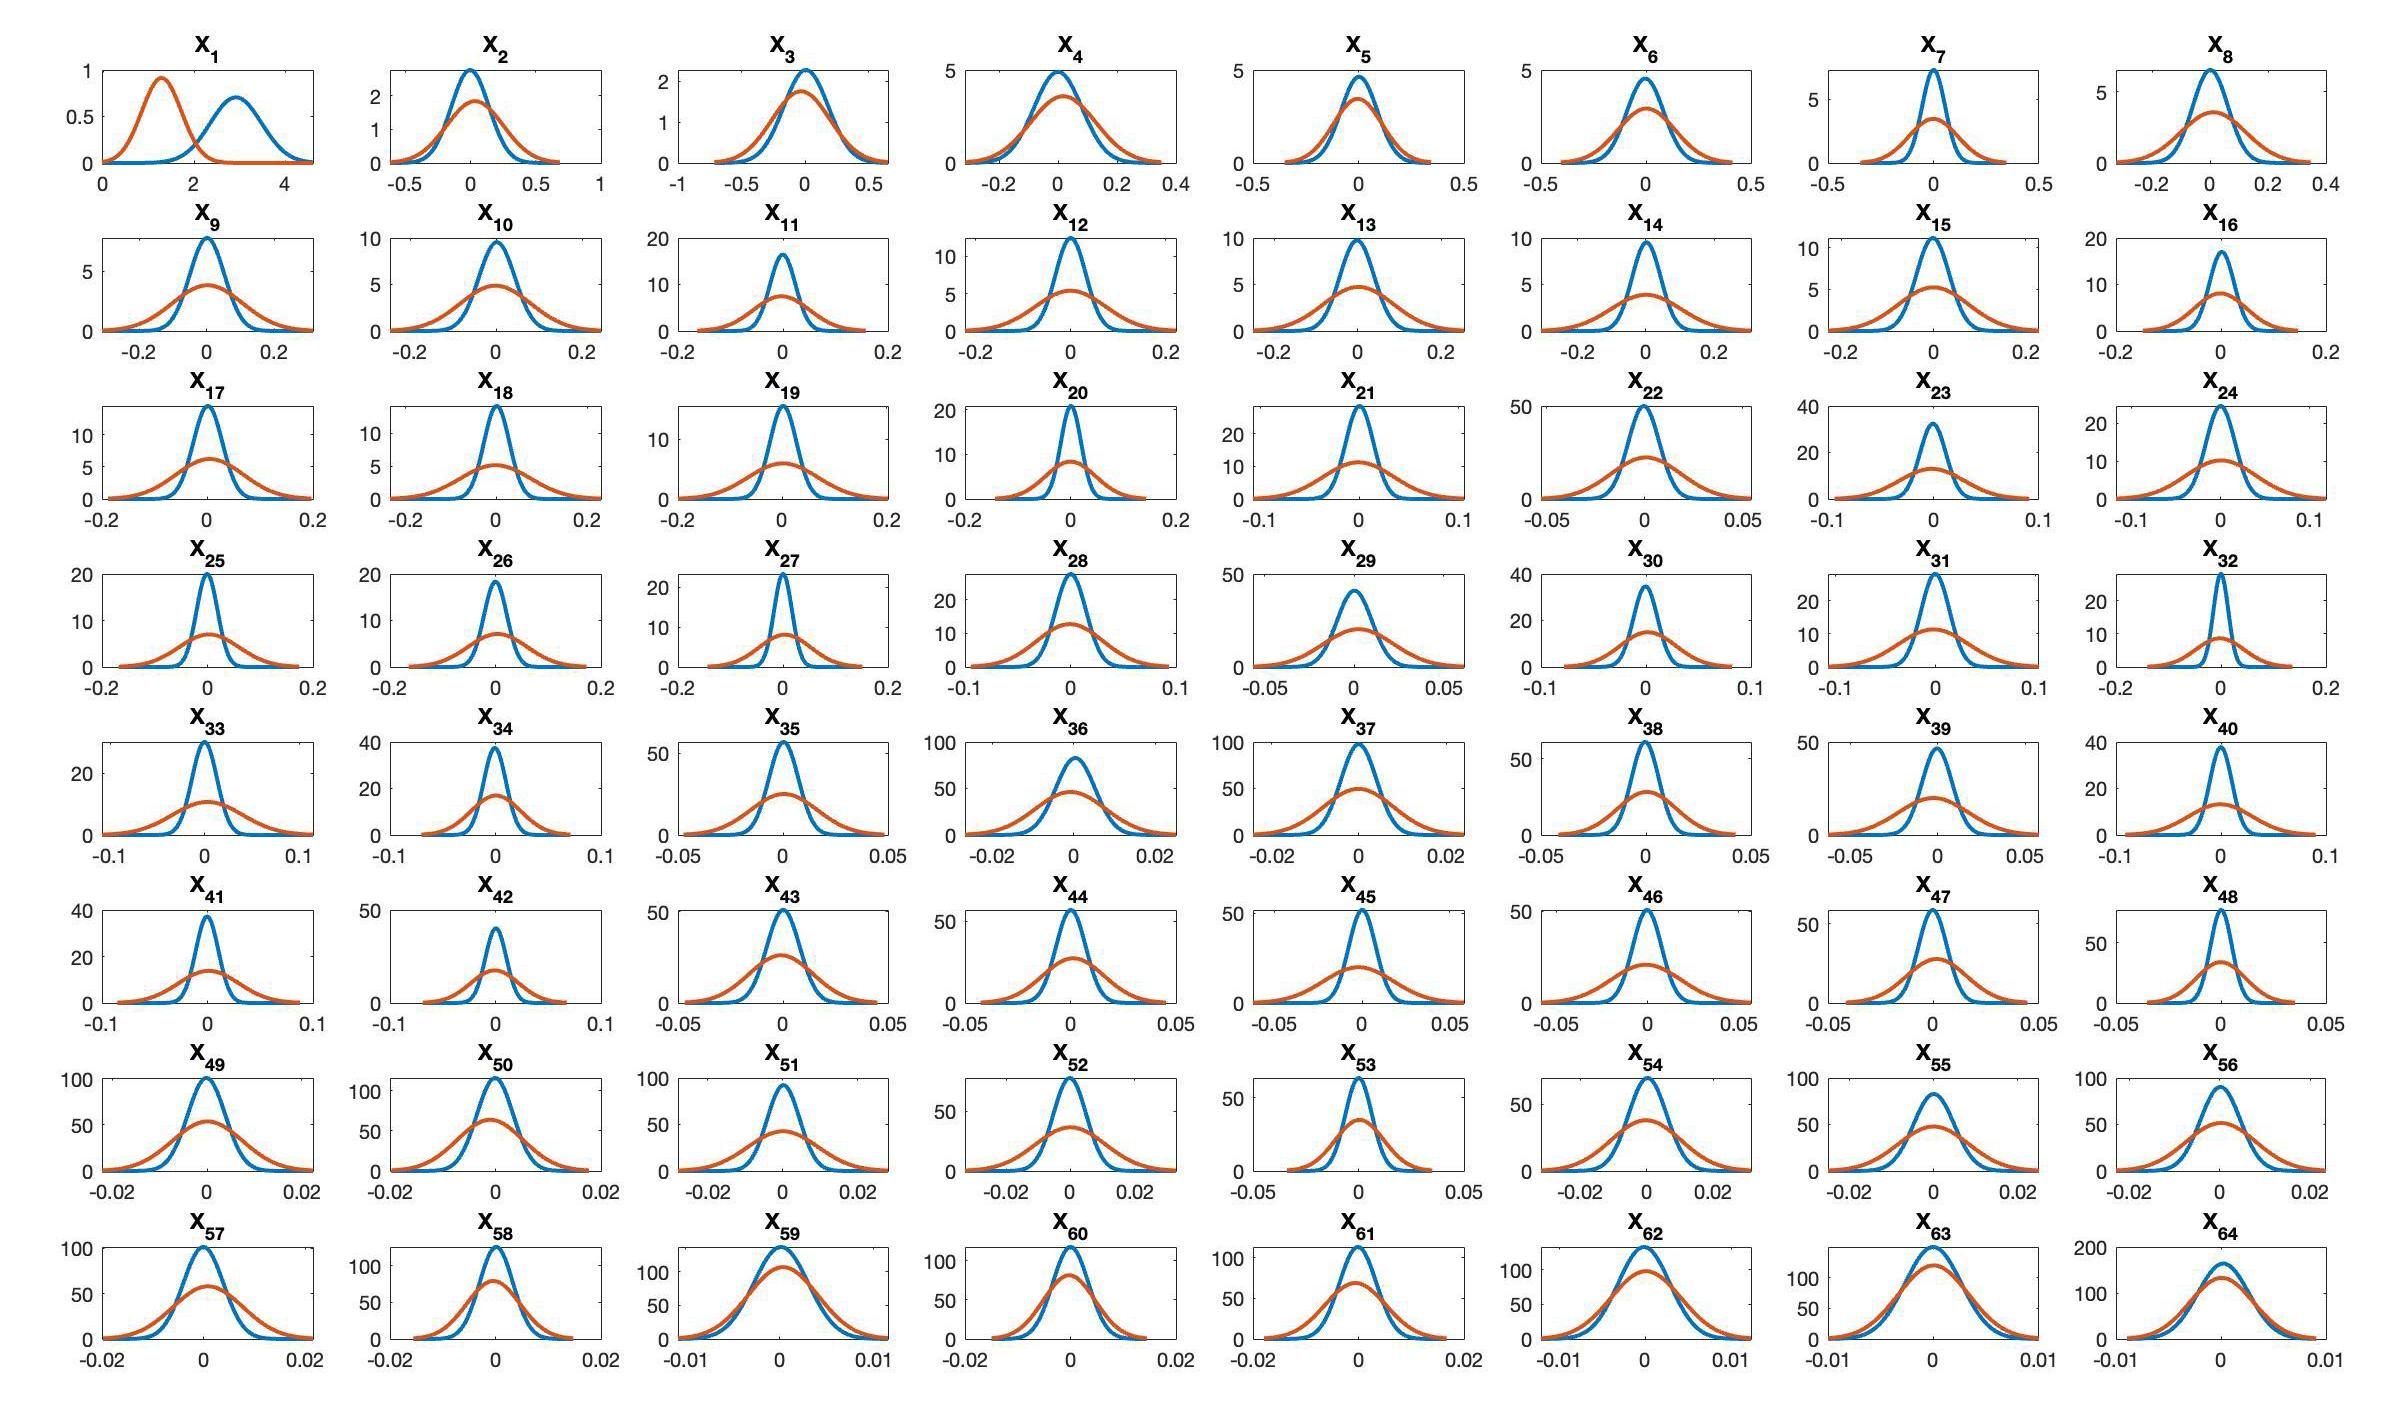
\includegraphics[width=\textwidth]{feature_plots}
\end{center}

By visual inspection, we pick $\{1, 25, 27, 32, 33, 45, 46, 48\}$ to be the best $8$ features because the two distributions appear to have less ambibuous decision ranges.
\begin{center}
  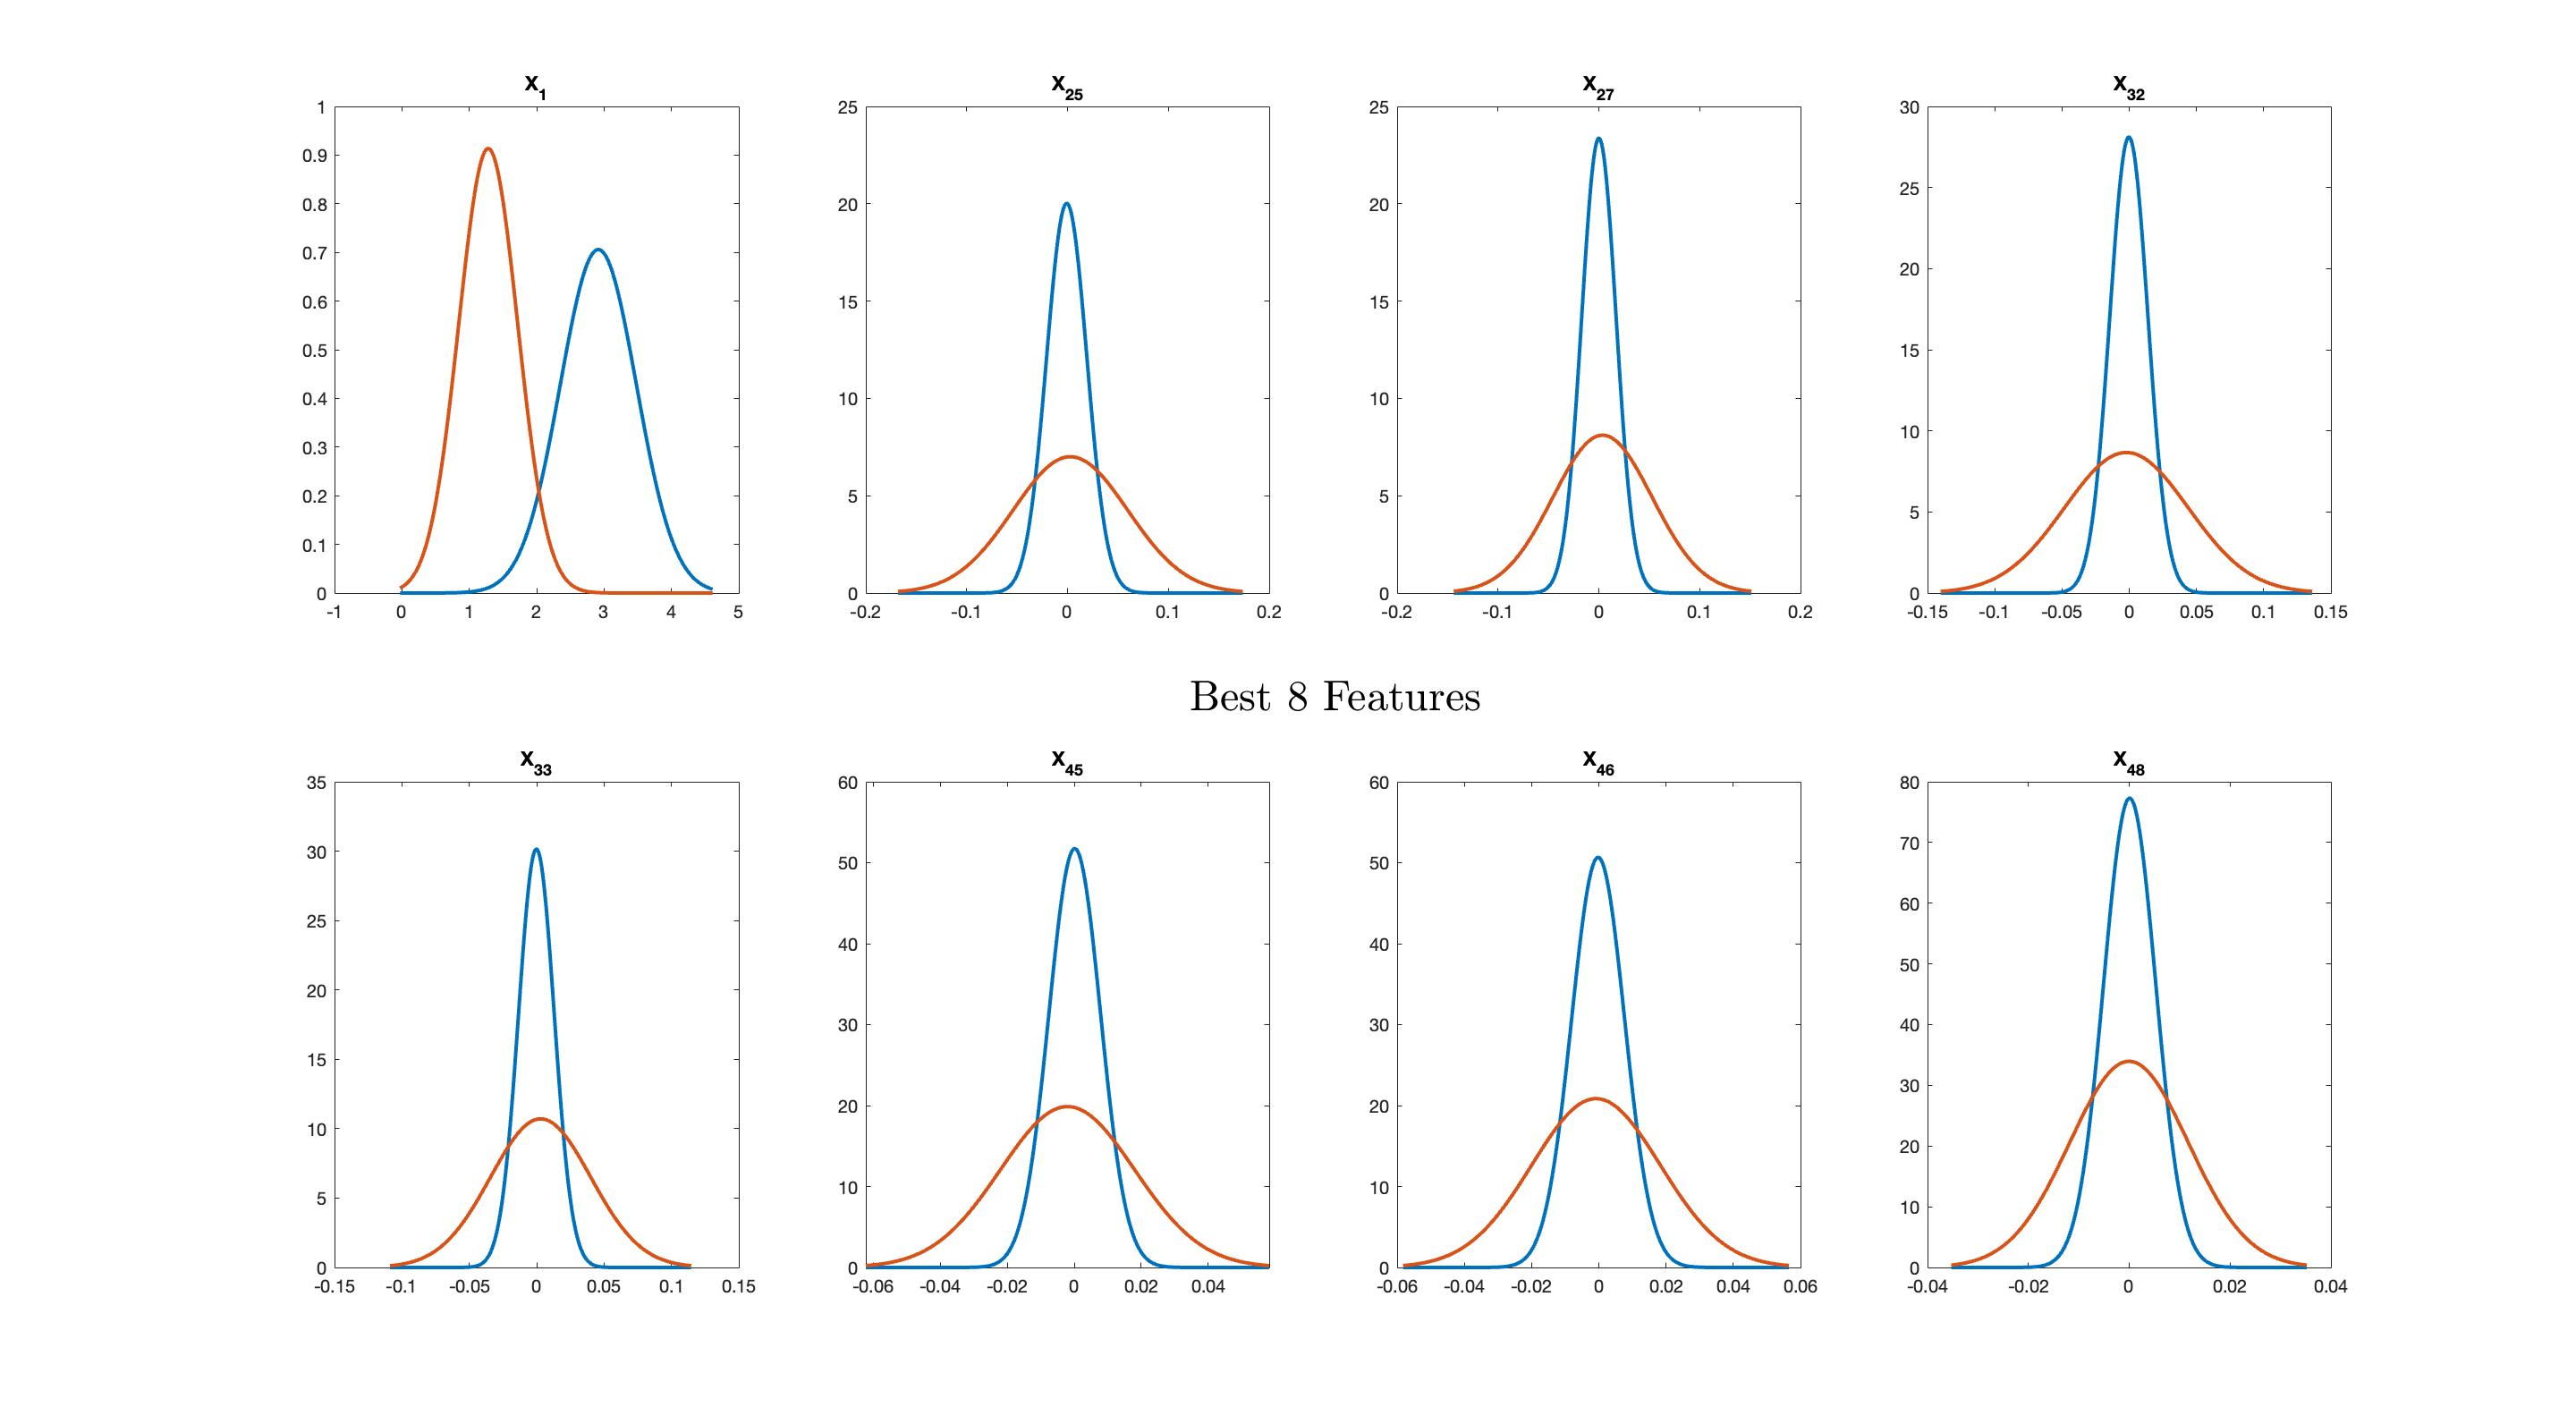
\includegraphics[width=\textwidth]{best8}
\end{center}
Conversely, we pick $\{2, 3, 4, 59, 60, 62, 63, 64\}$ to be the worst $8$ features, as the two distributions are highly overlapped.
\begin{center}
  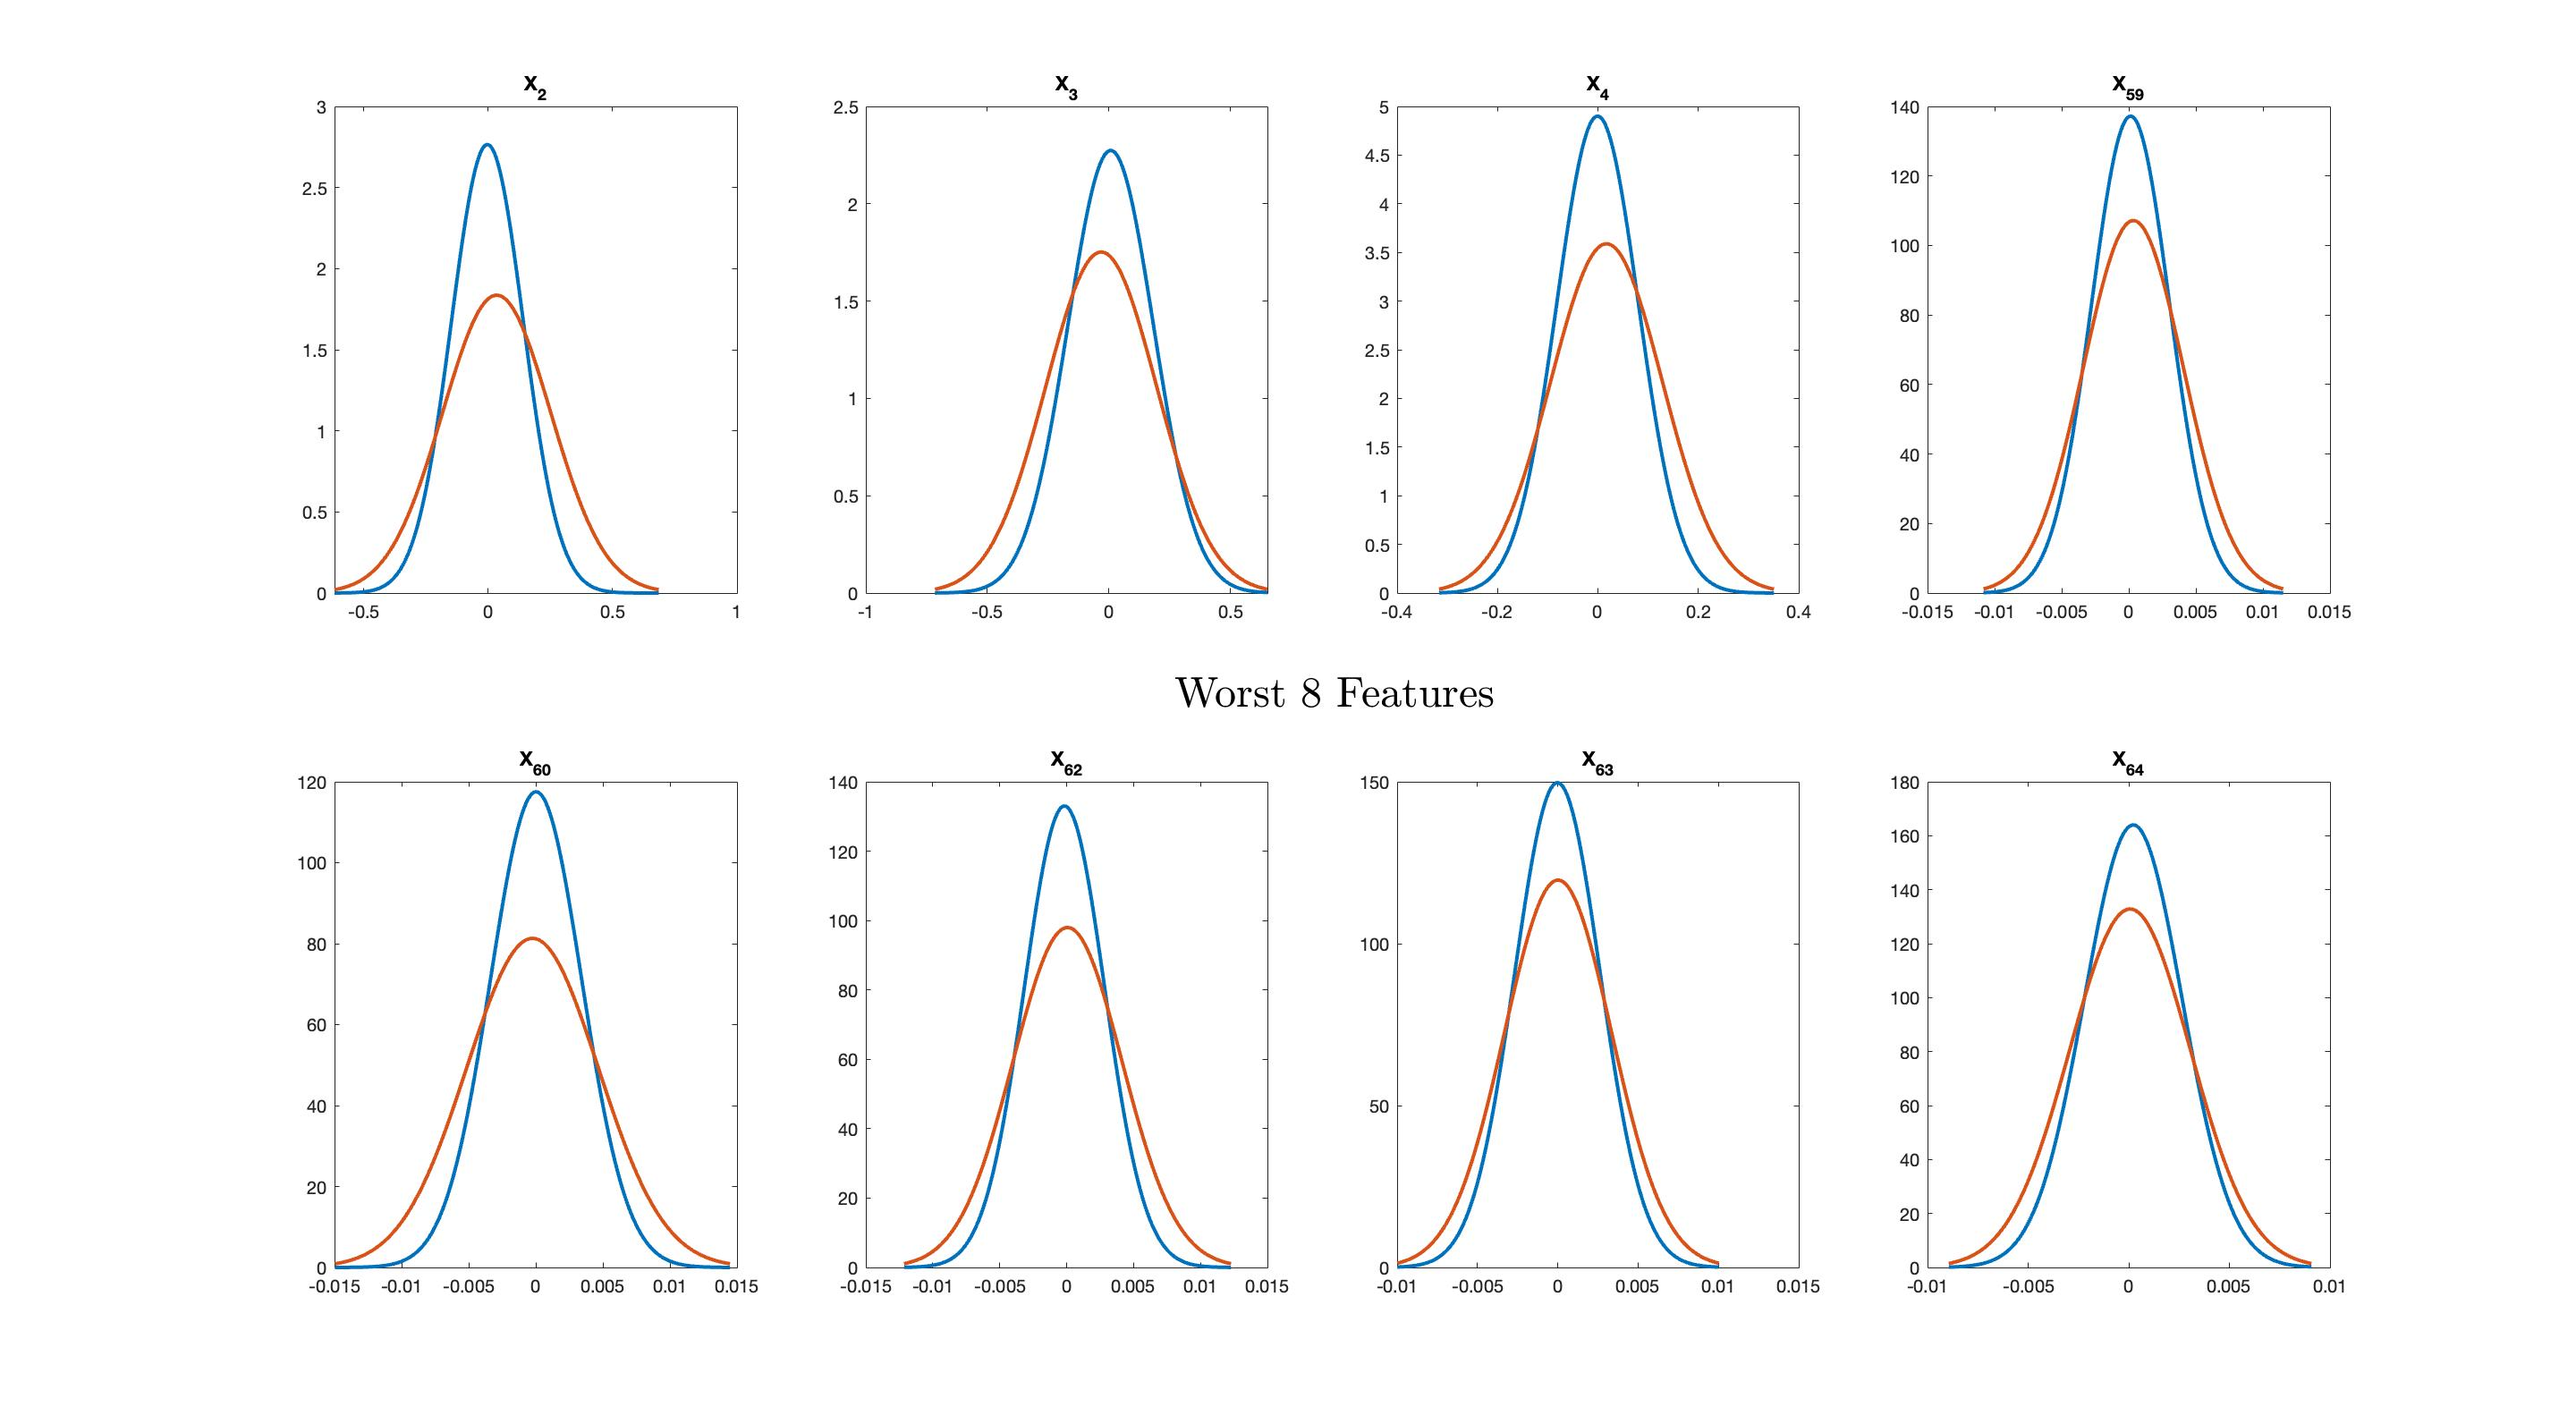
\includegraphics[width=\textwidth]{worst8}
\end{center}

\pagebreak

\section*{Part C}

Compute the Bayesian decision rule and classify the locations of the cheetah image using (i) the
64-dimensional Gaussians, and (ii) the 8-dimensional Gaussians associated with the best 8 features. For
the two cases, plot the classification masks and compute the probability of error by comparing with
cheetah mask.bmp. Can you explain the results?
\\

\textbf{\large Solution}

The following are the results of (i) and (ii).
\begin{center}
  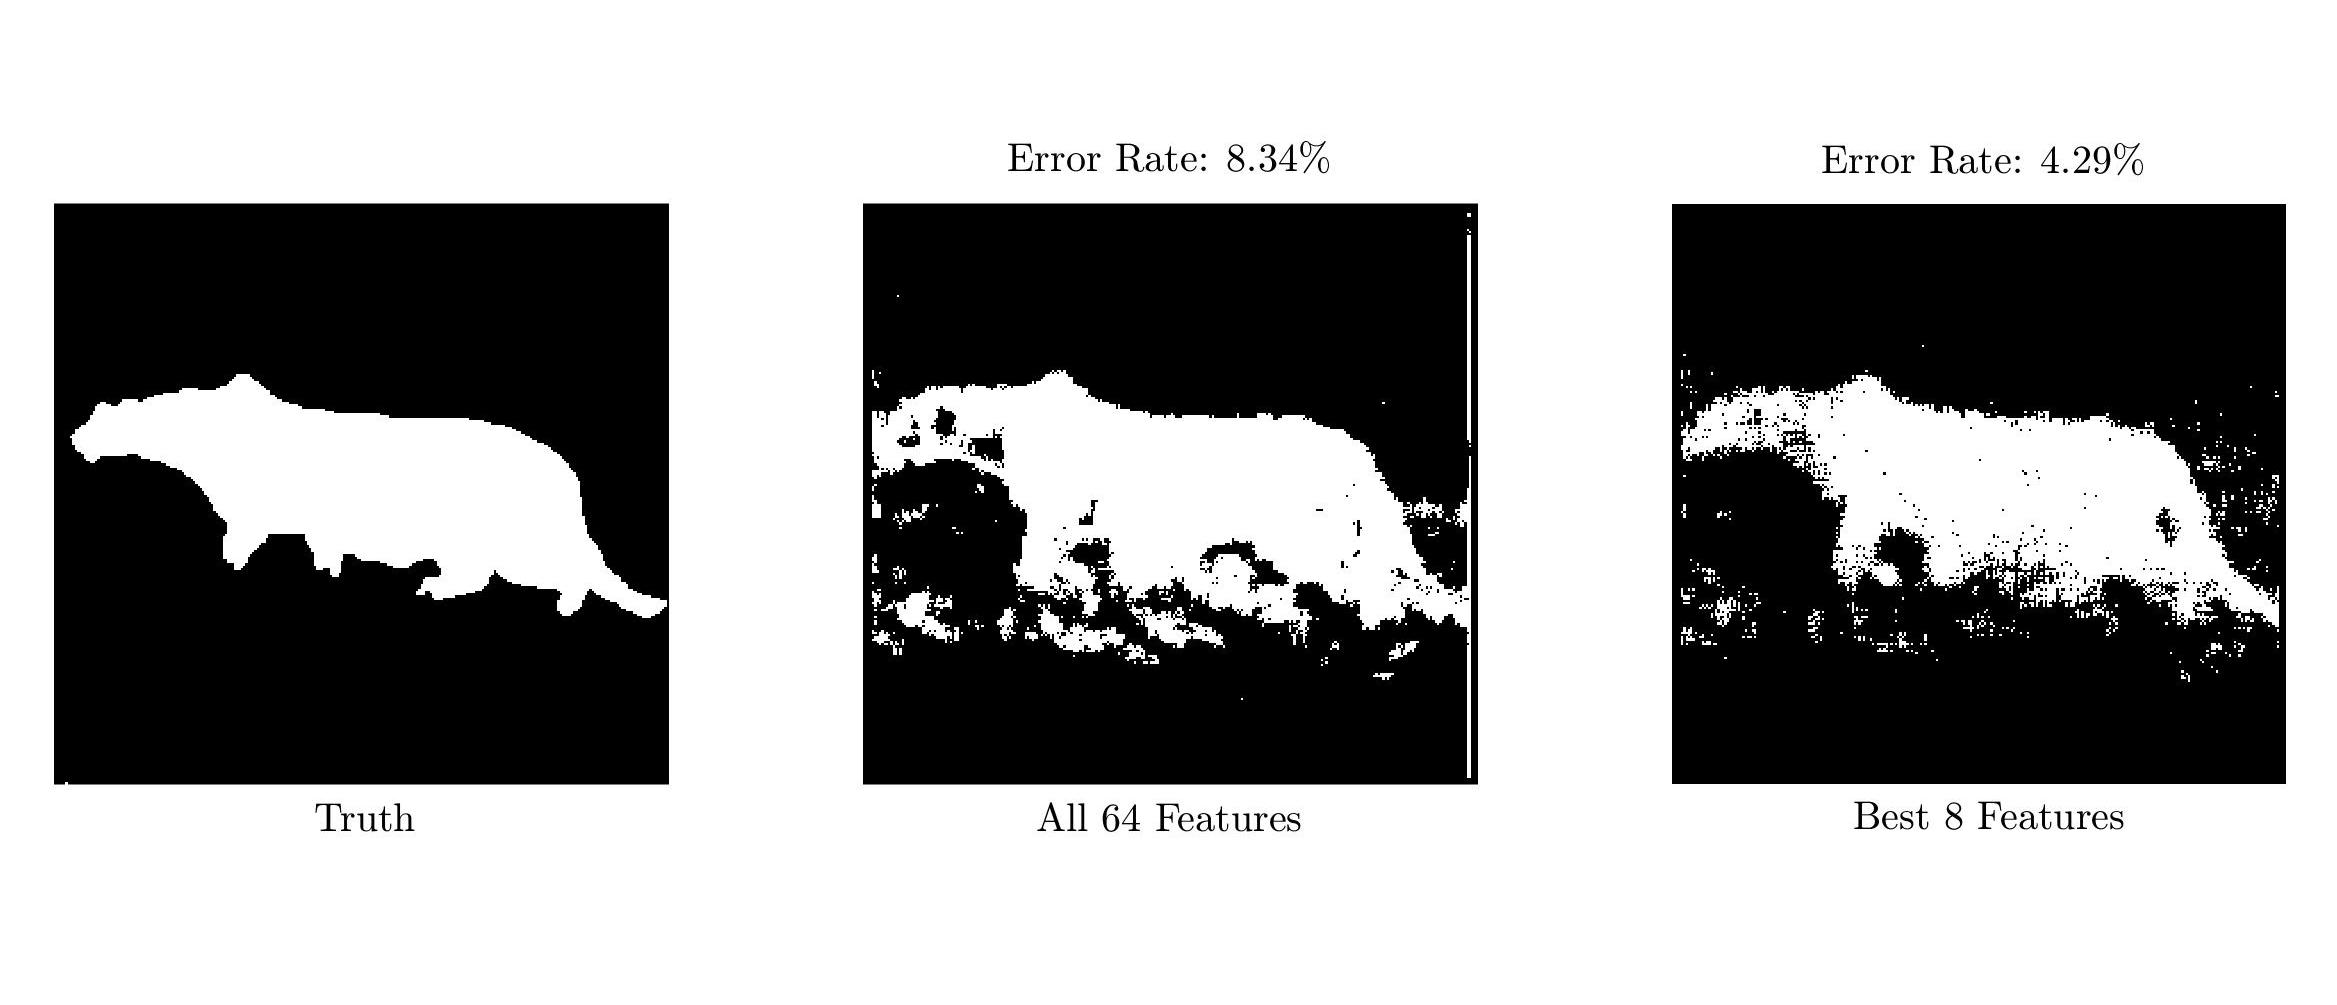
\includegraphics[width=\textwidth]{result}
\end{center}

Overall, (ii) exhibits a better performance comparing to (i). 
The reason might be that we have removed ambiguous features that have highly overlapping distributions between the two classes, e.g. the worst 8 features listed in part B, which could cause confusion to our decision.
In other words, we have filtered out the features that possibly possess high bayes risks, and thus we obtain an enhanced result.

\pagebreak

\section*{MATLAB Code}

\textbf{\large main.m}

\begin{lstlisting}[language=Matlab]
load('../dataset/TrainingSamplesDCT_8.mat');
zigzag = load('../dataset/Zig-Zag Pattern.txt');
cheetah = imread('../dataset/cheetah.bmp');
cheetah_mask = imread('../dataset/cheetah_mask.bmp');
target = im2double(cheetah);
mask = im2double(cheetah_mask);

training_BG = TrainsampleDCT_BG;
training_FG = TrainsampleDCT_FG;

zigzag = zigzag + 1;

[row_BG, col_BG] = size(training_BG);
[row_FG, col_FG] = size(training_FG);
[row_TG, col_TG] = size(target);

prior_BG = row_BG / (row_BG + row_FG);
prior_FG = row_FG / (row_BG + row_FG);

% pick cheetah if (p(x | grass) / p(x | cheetah)) < threshold
threshold = prior_FG / prior_BG;

mean_FG = zeros(1, 64);
mean_BG = zeros(1, 64);
cov_FG = zeros(64, 64);
cov_BG = zeros(64, 64);

for r = 1:row_FG
    cov_FG = cov_FG + training_FG(r,:)' * training_FG(r,:);
    mean_FG = mean_FG + training_FG(r,:);
end

for r = 1:row_BG
    cov_BG = cov_BG + training_BG(r,:)' * training_BG(r,:);
    mean_BG = mean_BG + training_BG(r,:);
end

mean_FG = mean_FG / row_FG;
mean_BG = mean_BG / row_BG;
cov_FG = (cov_FG / row_FG) - mean_FG' * mean_FG;
cov_BG = (cov_BG / row_BG) - mean_BG' * mean_BG;

figure;

for k = 1:64
    subplot(8, 8, k);
    x = linspace(min(mean_FG(k) - 3 * sqrt(cov_FG(k, k)), ...
        mean_BG(k) - 3 * sqrt(cov_BG(k, k))), ...
        max(mean_FG(k) + 3 * sqrt(cov_FG(k, k)), ...
        mean_BG(k) + 3 * sqrt(cov_BG(k, k))), 1000);
    p_BG = (1/(sqrt(2*pi * cov_BG(k, k)))) * exp(-0.5 * ...
        ((x - mean_BG(1,k)).^2/cov_BG(k, k)));
    p_FG = (1/(sqrt(2*pi * cov_FG(k, k)))) * exp(-0.5 * ...
        ((x - mean_FG(1,k)).^2/cov_FG(k, k)));
    plot(x, p_BG, 'LineWidth', 2);
    hold on;
    plot(x, p_FG, 'LineWidth', 2);
    title("X_{" + k + "}");
end

figure;
for i = 1:8
    subplot(2, 4, i);
    k = best8(i);
    x = linspace(min(mean_FG(k) - 3 * sqrt(cov_FG(k, k)), ...
        mean_BG(k) - 3 * sqrt(cov_BG(k, k))), ...
        max(mean_FG(k) + 3 * sqrt(cov_FG(k, k)), ...
        mean_BG(k) + 3 * sqrt(cov_BG(k, k))), 1000);
    p_BG = (1/(sqrt(2*pi * cov_BG(k, k)))) * exp(-0.5 * ...
        ((x - mean_BG(1,k)).^2/cov_BG(k, k)));
    p_FG = (1/(sqrt(2*pi * cov_FG(k, k)))) * exp(-0.5 * ...
        ((x - mean_FG(1,k)).^2/cov_FG(k, k)));
    plot(x, p_BG, 'LineWidth', 2);
    hold on;
    plot(x, p_FG, 'LineWidth', 2);
    title("X_{" + k + "}");
end

figure;
for i = 1:8
    subplot(2, 4, i);
    k = worst8(i);
    x = linspace(min(mean_FG(k) - 3 * sqrt(cov_FG(k, k)), ...
        mean_BG(k) - 3 * sqrt(cov_BG(k, k))), ...
        max(mean_FG(k) + 3 * sqrt(cov_FG(k, k)), ...
        mean_BG(k) + 3 * sqrt(cov_BG(k, k))), 1000);
    p_BG = (1/(sqrt(2*pi * cov_BG(k, k)))) * exp(-0.5 * ...
        ((x - mean_BG(1,k)).^2/cov_BG(k, k)));
    p_FG = (1/(sqrt(2*pi * cov_FG(k, k)))) * exp(-0.5 * ...
        ((x - mean_FG(1,k)).^2/cov_FG(k, k)));
    plot(x, p_BG, 'LineWidth', 2);
    hold on;
    plot(x, p_FG, 'LineWidth', 2);
    title("X_{" + k + "}");
end

best8 = [1 25 27 32 33 45 46 48];
worst8 = [2 3 4 59 60 62 63 64];

E = zeros(8, 64);

for i = 1:8
    E(i, best8(i)) = 1;
end

mean8_FG = zeros(1, 8);
mean8_BG = zeros(1, 8);
cov8_FG = zeros(8, 8);
cov8_BG = zeros(8, 8);

for r = 1:row_FG
    v = E * training_FG(r,:)';
    cov8_FG = cov8_FG + v * v';
    mean8_FG = mean8_FG + v';
end

for r = 1:row_BG
    v = E * training_BG(r,:)';
    cov8_BG = cov8_BG + v * v';
    mean8_BG = mean8_BG + v';
end

mean8_FG = mean8_FG / row_FG;
mean8_BG = mean8_BG / row_BG;
cov8_FG = (cov8_FG / row_FG) - mean8_FG' * mean8_FG;
cov8_BG = (cov8_BG / row_BG) - mean8_BG' * mean8_BG;

A_64 = zeros(row_TG, col_TG);
A_8 = zeros(row_TG, col_TG);

for r = 5:row_TG-3
    for c = 5:col_TG-3
        block = target(r - 4:r + 3, c - 4:c + 3);
        dctBlock = dct2(block);
        X = zeros(1, 64);
        for i = 1:8
            for j = 1:8
                X(zigzag(i, j)) = dctBlock(i, j);
            end
        end
        A_64(r, c) = int8(mvn(X, mean_BG, cov_BG)/ ...
            mvn(X, mean_FG, cov_FG) <= threshold);
        A_8(r, c) = int8(mvn(X * E', mean8_BG, cov8_BG)/ ...
            mvn(X * E', mean8_FG, cov8_FG) <= threshold);
    end
end

figure;

subplot(1, 3, 1);
imagesc(mask);
axis off
colormap(gray(255));
axis equal tight;

subplot(1, 3, 2);
imagesc(A_64);
axis off
colormap(gray(255));
axis equal tight;

subplot(1, 3, 3);
imagesc(A_8);
axis off
colormap(gray(255));
axis equal tight;

error64 = 0;
error8 = 0;
for r = 1:row_TG
    for c = 1:col_TG
        if (A_64(r, c) ~= mask(r, c))
            error64 = error64 + 1;
        end

        if (A_8(r, c) ~= mask(r, c))
            error8 = error8 + 1;
        end
    end
end

error_rate64 = error64 / (row_TG * col_TG);
error_rate8 = error8 / (row_TG * col_TG);
disp(error_rate64);
disp(error_rate8);
\end{lstlisting}

\textbf{\large mvn.m}

\begin{lstlisting}
function result = mvn(x, mean, cov)
  [~, dim] = size(mean);
  d = (x - mean) * inv(cov) * (x - mean)';
  c = 1/sqrt((2 * pi)^dim * det(cov));
  result = c * exp(-0.5 * d);
end
\end{lstlisting}

\end{document}